\documentclass{article}
\usepackage[T1]{fontenc}
\usepackage[utf8]{inputenc}
\usepackage{ismir,amsmath,cite,url}
\usepackage{graphicx,booktabs,array}
\usepackage[bookmarks=false,hidelinks]{hyperref}

\renewcommand{\permission}{}
\title{Individual Progress Report \\ Major/Minor Errors in Guitar Chord Recognition}
\oneauthor{Christopher Xu}{CSC575  \\ November 2026}
\def\authorname{C. Xu}
% Tables checked against saved development and fast-tempo comparisons.
\newcommand{\RootResults}{%
\begin{table}[t]
\centering
\small
\setlength{\tabcolsep}{2.7pt}
\begin{tabular}{@{}lrrrrr@{}}
\toprule
 & \multicolumn{2}{c}{Dev. (119)} & \multicolumn{3}{c}{Fast IDMT (64)} \\
Method & Chord & Root & Chord & Root & Time (s)\\
\midrule
Long STFT & 71.97 & 74.48 & 64.70 & 73.91 & 9.49\\
Note NNLS & 78.37 & 80.15 & 66.95 & 78.45 & 44.37\\
Projection & 78.02 & 79.54 & 67.80 & 78.32 & 10.43\\
\bottomrule
\end{tabular}
\caption{Decoded duration-weighted accuracies (\%); chord includes reference $N$, root excludes it. Note models use fundamental-only profiles. Time covers full inference on 64 fast files.}
\label{tab:root}
\end{table}
}
\newcommand{\ProgressTable}{%
\begin{table}[htbp]
\centering
\small
\begin{tabular}{@{}ll>{\raggedright\arraybackslash}p{4.9cm}@{}}
\toprule
PI & Level & Status and evidence \\
\midrule
O1.1 & Basic & Done: aligned labels and predictions (\S\ref{sec:method}, Fig.~\ref{fig:quality}b).\\
O1.2 & Basic & Done: short, long and CQT comparison (\S\ref{sec:fusion}).\\
O1.3 & Expected & Done: fixed/adaptive fusion (\S\ref{sec:fusion}).\\
O1.4 & Expected & Done: playback and timed CSV (Fig.~\ref{fig:demo}).\\
O1.5 & Advanced & Open: reassigned-spectrum comparison.\\
O2.1 & Basic & Done: saved split, settings and versions (\S\ref{sec:individual}).\\
O2.2 & Basic & Done: duration, coverage and boundary metrics (\S\ref{sec:data}, \S\ref{sec:comparison}).\\
O2.3 & Expected & Done: accuracy, timing and error cases (Table~\ref{tab:root}, \S\ref{sec:comparison}, Figs.~\ref{fig:demo}--\ref{fig:quality}).\\
O2.4 & Expected & Done for this report; final version remains (\S2, \S4, \S\ref{sec:future}).\\
O2.5 & Advanced & Open: uncertainty analysis with valid grouping.\\
\bottomrule
\end{tabular}
\caption{Original proposal indicators. Basic and expected work is complete for this progress report; the final report remains pending.}
\label{tab:progress}
\end{table}
}

\sloppy
\begin{document}
\maketitle


\begin{abstract}
A working guitar chord recognizer converts audio into timed major/minor labels, with interval playback and CSV export for inspection. This report presents comparisons of spectral features, fusion and note representations. Window fusion offered little benefit; note projection improved overall chord and root accuracy over the long-window baseline. Projection also increased decoded same-root quality errors, concentrated in one seventh-chord recording. These findings extend the original system-building objectives into a controlled study of third strength and seventh-tone presence, comparing template scores with calibrated decoding.
\end{abstract}

\section{Introduction}
Automatic chord recognition assigns harmonic labels to intervals of audio. Systems typically combine pitch features, chord models and temporal decoding\ \cite{mcvicar2014,pauwels2019,mueller2021fmp}. This project implements that pipeline for guitar recordings, with playback and timed label export. The original objectives were to build a multi-resolution recognizer and evaluate its accuracy, errors and runtime.

A major/minor label identifies a root and a quality: C major and C minor share C and G, but their thirds are E and E$\flat$. Evaluation labels can omit sounding notes: C7 (C--E--G--B$\flat$) reduces to C major, and Cm7 (C--E$\flat$--G--B$\flat$) to C minor. Vocabulary reduction and annotation ambiguity therefore affect error interpretation\ \cite{humphrey2015,koops2019}.

The completed comparisons improved root recognition but exposed a quality-error increase. Long-window STFT chroma (Long STFT) and note projection had similar raw same-root quality-error durations: 49.58 and 49.64\,s. Shared decoding reduced these to 19.07 and 27.41\,s. The added decoded errors were concentrated in a seventh-chord recording, motivating a closer look at feature evidence and temporal decisions.

Our research question is: \textbf{How does an added seventh affect major/minor recognition as third strength varies?} Here, third strength means amplitude relative to fixed root and fifth components; pitch remains unchanged.

\section{Related Work}
Ding et al.\ \cite{ding2026} compare estimated pitches with score-derived inputs in a learned two-stage recognizer. ChordFormer\ \cite{akram2026} predicts chord components and examines quality confusions with correct roots. Poltronieri et al.\ \cite{poltronieri2025} use component predictions and consonance-based training-label smoothing; one ablation improves root accuracy while reducing major/minor accuracy. These studies motivate separating acoustic evidence, root errors and quality errors.

Mauch and Dixon\ \cite{mauch2010} estimate note activations with harmonic profiles and non-negative least squares (NNLS). Reassigned spectra\ \cite{khadkevich2013} and learned chroma\ \cite{korzeniowski2016} provide alternative pitch representations. 

Cho et al.\ \cite{cho2010} find that suitable switching penalties differ across chord models. Duration models\ \cite{korzeniowski2018} and event-based prediction\ \cite{kim2026} address sequence structure more explicitly. These results support retaining raw predictions alongside calibrated decoding. Phan et al.'s released model\ \cite{phan2026} offers a later comparison.

\section{Method and Evaluation}
\label{sec:method}
\subsection{Spectral and note representations}
Audio is converted to mono at 22,050\,Hz. Short-time Fourier transform (STFT) chroma uses 2,048- or 8,192-sample Hann windows; constant-Q transform (CQT) chroma uses 12 bins per octave. All features share a 512-sample hop, tuning estimate, MIDI range 36--95, C-first pitch classes and per-frame L2 normalization. Fixed fusion takes a weighted average of short/long chroma; adaptive fusion increases the short-window weight around detected changes.

The note-based candidates use the long-window magnitude spectrum $y_t$. Dictionary columns $d_n$ are tuned Hann-windowed sine responses. Non-negative least squares (NNLS) fits notes jointly; projection fits them separately:
\begin{equation}
 \hat a_t=\arg\min_{a\geq0}\|y_t-Da\|_2^2,\qquad
 p_n(t)=\frac{d_n^\top y_t}{d_n^\top d_n}.
 \label{eq:notes}
\end{equation}
Activations are folded by pitch class and normalized. The selected candidates use fundamental-only profiles on a linear-frequency magnitude spectrum, unlike Mauch and Dixon's harmonic dictionary and standardized log-frequency spectrum\ \cite{mauch2010}. Harmonic profiles were also tested.

\subsection{Template scoring and temporal decoding}
Each of the 24 major/minor templates assigns weight $1/\sqrt{3}$ to its root, third and fifth, and zero elsewhere. For nonzero, nonnegative chroma $c$ before normalization, the same-root score difference is
\begin{equation}
 \Delta_C(c)=s(C\mathrm{maj})-s(C\mathrm{min})
 =\frac{c_E-c_{E^\flat}}{\sqrt{3}\,\|c\|_2}.
 \label{eq:margin}
\end{equation}
Adding B$\flat$ while holding the other components fixed shrinks a nonzero $|\Delta_C|$ without reversing its sign. Other roots can still compete: for ideal Cm7, C minor and E$\flat$ major have equal scores whenever the root and seventh activations match, regardless of third strength.

Frames at least 45\,dB below peak root-mean-square amplitude receive the no-chord label $N$; otherwise raw predictions maximize template scores. Viterbi decoding selects
\begin{equation}
 \hat s_{1:T}=\arg\max_{s_{1:T}}\left[
 \sum_{t=1}^{T}e_t(s_t)-\lambda\sum_{t=2}^{T}\mathbf{1}_{s_t\ne s_{t-1}}\right],
 \label{eq:decode}
\end{equation}
where $e_t$ is the template score subject to the silence rule. Identical consecutive states become intervals. All representations retain $\lambda=4$ from development; L2 normalization does not equalize score margins or smoothing strength. The implementation uses Python, NumPy/SciPy, librosa\ \cite{mcfee2015}, SoundFile and mir\_eval\ \cite{raffel2014}.

\subsection{Data, selection and metrics}
\label{sec:data}
GuitarSet v1.1.0\ \cite{guitarset} supplies microphone accompaniment recordings and performed chord labels. Excluding two files with timing errors leaves 119 development recordings from progression families 1 and 2; family 3 is excluded from selection. All variants of a family stay together.

IDMT-SMT-Guitar\ \cite{idmt} subset 4 supplies acoustic microphone recordings: 64 slow-tempo files for fusion and 64 fast-tempo files for note representations. These sets share piece IDs. Settings were fixed before scoring; error analysis is exploratory. The fast set totals 29.77 minutes: 59.56\% scoreable, 27.07\% unannotated leading/trailing audio and 13.37\% unsupported labels. Chord and root scores use 59 and 58 files, respectively; all 64 enter runtime and coverage totals.

Duration-weighted chord accuracy uses mir\_eval's major/minor comparison, retaining $N$ and excluding unsupported labels and gaps. Root accuracy excludes reference $N$ but counts predicted $N$ as wrong. Same-root quality errors have the correct root and wrong major/minor type. IDMT labels span annotated beats; \texttt{NC} is mapped to $N$ as a project convention because the guide does not define it. Boundary F1 uses one-to-one matching within 100\,ms inside contiguous scoreable spans, excluding gap edges.

Inference times cover loading through interval construction, including resampling, tuning, features, dictionary construction, fitting and decoding. Measurements use an Intel Core Ultra 9 285K CPU, one BLAS/OpenMP thread and no feature cache; warm-up, scoring and writing are excluded. Run records preserve configurations, input hashes and per-recording accuracy and runtime.\footnote{\url{https://github.com/cxMoonGlade/CSC-575}}

\section{Progress and Preliminary Results}
\subsection{Spectral features and fusion}
\label{sec:fusion}
On 119 development recordings with shared decoding, short STFT and CQT reached 64.56\% and 64.95\% chord accuracy, versus 71.97\% for Long STFT. Adaptive fusion reached 71.66\%; the selected fixed weight was zero, reproducing Long STFT. A later 4,096/8,192-sample blend reached 72.22\%, but on slow IDMT the frozen blend scored 65.56\%, versus 65.73\% for Long STFT. This weak transfer prompted the move to note representations.

\subsection{Note representations and demonstration}
\label{sec:comparison}
Note representations improved development accuracy (Table~\ref{tab:root}); fundamental-only NNLS outperformed the tested harmonic profiles.

\RootResults

On fast IDMT, projection gained 3.10 points in chord accuracy and 4.41 points in root accuracy over Long STFT. It improved 30 scoreable recordings, tied 13 and worsened 16; the rock/blues aggregate fell by 6.18 points. Boundary F1 rose from 27.27\% to 28.90\%. NNLS identified slightly more roots but made more quality errors and took over four times as long as projection. Projection is the current demonstration method.

The player supports timeline seeking and interval playback; predictions are also saved as timestamped CSV. Figure~\ref{fig:demo} shows a corrected root error in a development recording.

% The compact view is captured from the existing player with unchanged predictions.
\begin{figure}[t]
\centering
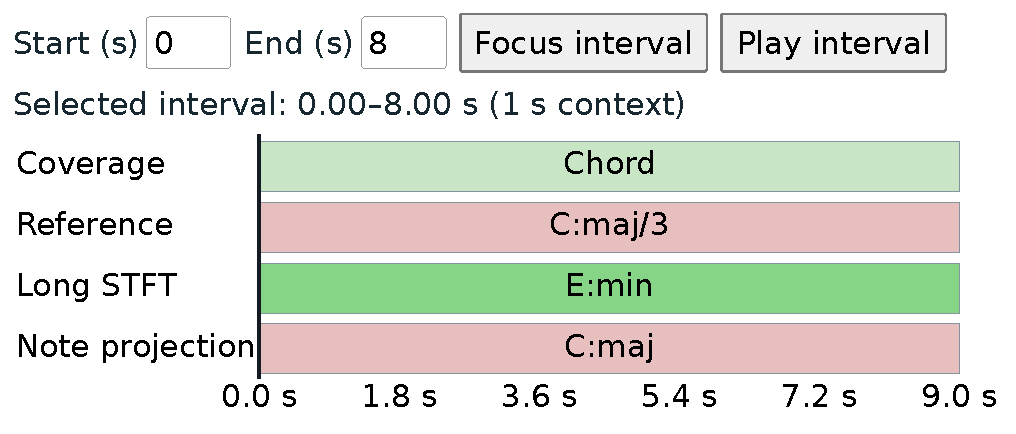
\includegraphics[width=\columnwidth]{figures/demo_progress.pdf}
\caption{Compact playback view of a GuitarSet development example, \texttt{01\_Funk1-97-C\_comp}. Projection corrects Long STFT's E-minor error. The CSV begins \texttt{0.000,}\allowbreak\texttt{9.973,}\allowbreak\texttt{C:maj}: start, end (seconds), label, rounded for display.}
\label{fig:demo}
\end{figure}

\subsection{Where the quality errors changed}
\label{sec:errors}
The nearly equal raw error totals conceal different locations: 39.29\,s were shared, with 10.29\,s unique to Long STFT and 10.35\,s unique to projection. After decoding, projection introduced 10.60\,s of same-root quality errors where Long STFT was correct, and corrected 2.26\,s of Long STFT quality errors. Some quality errors therefore replaced correct labels.

Quality errors fell on triad references but rose on references with additional tones (Fig.~\ref{fig:quality}); these groups ignore the bass field. The overall increase was 8.34\,s, with \texttt{rock\_6} contributing 9.89\,s. Its A7/D7/E7 references reduce to major. A frame-score check found that the correct major template outscored its minor counterpart during 7.85 of projection's 9.89\,s of decoded quality errors in this file. The mean margin over these errors was nevertheless negative: score magnitudes as well as durations matter. Physical third strength remains unmeasured.

\begin{figure}[t]
\centering
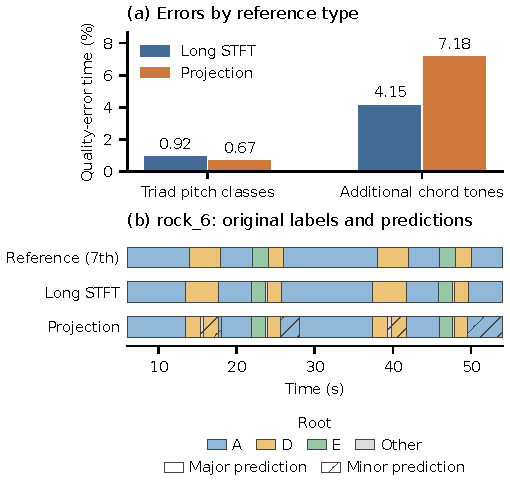
\includegraphics[width=\columnwidth]{figures/quality_diagnostic.pdf}
\caption{(a) Decoded quality-error time divided by supported chord time: 612.93\,s for triads, 324.01\,s for additional tones; $N$ excluded. (b) \texttt{rock\_6}, selected after evaluation for the largest quality-error increase. A7/D7/E7 references reduce to major. Colours show roots; grey groups other roots. Solid/hatched predictions indicate major/minor.}
\label{fig:quality}
\end{figure}

\section{Individual Progress: Christopher Xu}
\label{sec:individual}
I implemented the system (O1), evaluation (O2) and demonstration (Table~\ref{tab:progress}). The split and settings are saved in \texttt{configs/}; the requirements lockfile and run records preserve software versions.

\ProgressTable

\section{Discussion and Remaining Work}
\label{sec:future}
The score diagnostic makes calibration the next priority. Each representation's penalty will be selected by duration-weighted chord accuracy on the 119 GuitarSet development recordings and frozen before an exploratory fast-IDMT reassessment.

The controlled study will compare ideal vectors and paired audio, holding root/fifth amplitudes at 1, varying the third over \{1, 0.5, 0.25\}, and adding a minor seventh at amplitude 0 or 1. Tied ideal maximizers will be recorded within a fixed numerical tolerance, alongside single-label errors. Synthetic development and confirmation sequences will contain root and same-root quality changes, with source variants kept in one split. Each representation's penalty will be chosen by synthetic development chord accuracy and frozen for confirmation. Major/minor conditions and root/quality errors will be separated, comparing raw, shared-penalty and calibrated predictions. Departures from ideal margins will prompt feature inspection; persistent root competition will motivate revised templates. Stimulus controls are specified in the README.

\textbf{Basic final goals} are the reproducible comparisons and playback demonstration. \textbf{Expected goals} add the paired margin/error curves and calibrated decoding. \textbf{Advanced goals} add seventh-aware templates or a frozen recent model, guided by the results; confirmation on real guitar requires new pieces.

Working milestones are \textbf{Nov.~16--19}: calibrated comparisons, ideal scores and synthetic sequences; \textbf{Nov.~20--26}: paired margin/error curves; \textbf{Nov.~27--Dec.~3}: final report and demonstration.

\bibliography{references}
\end{document}
